
\documentclass[journal]{IEEEtran}
\IEEEoverridecommandlockouts
%%%%%%%%%%%%%%%%%%%%%%%%%%%%%%%%%%%%%%
%%%%%%%% PRINCIPALES PAQUETES %%%%%%%%
%%%%%%%%%%%%%%%%%%%%%%%%%%%%%%%%%%%%%%
\usepackage{fancyhdr}
\usepackage{graphicx}
\usepackage[spanish, es-tabla]{babel}
\usepackage[utf8]{inputenc}
\usepackage{color}
\usepackage{hyperref}
\usepackage{wrapfig}
\usepackage{array}
\usepackage{multirow}
\usepackage{adjustbox}
\usepackage{nccmath}
%\usepackage{anysize}
\usepackage{subfigure}
\usepackage{amsfonts,latexsym} % para tener disponibilidad de diversos simbolos
\usepackage{enumerate}
\usepackage{booktabs}
\usepackage{float}
\usepackage{threeparttable}
\usepackage{array,colortbl}
\usepackage{ifpdf}
\usepackage{rotating}
\usepackage{cite}
\usepackage{stfloats}
\usepackage{url}
\usepackage{listings}
%%%%%%%%%%%%%%%%%%%%%%%%%%%%%%%%%%%%%%%%%%%
%%% CREAR Y REESCRIBIR ALGUNOS COMANDOS %%%
%%%%%%%%%%%%%%%%%%%%%%%%%%%%%%%%%%%%%%%%%%%
\newcolumntype{P}[1]{>{\centering\arraybackslash}p{#1}}  %% Se crea un nuevo tipo de columna llamada P.
\newcommand{\tabitem}{~~\llap{\textbullet}~~}
\newcommand{\ctt}{\centering\scriptsize\textbf} %%\ctt abrevia el comando \centering\scriptsize\textbf
\newcommand{\dtt}{\scriptsize\textbf} %%\dtt abrevia el comando \scriptsize\textbf
\renewcommand\IEEEkeywordsname{Palabras clave}


\renewcommand\IEEEkeywordsa{Key words}
\renewcommand\abstracteee{Abstract}

%%%%%%%%%%%%%%%%%%%%%%%%%%%%%%%%%%%%%%%%%%%


% correct bad hyphenation here
\hyphenation{op-tical net-works semi-conduc-tor} %% Con este comando se especifican como pueden seprarse las sílabas adecuadamente en caso una palabra quede en dos lineas diferentes de texto

\graphicspath{ {Figs/} }  %%Ruta donde se encuentran las imágenes, que esté vacio indica que las imagenes están dentro de la misma carpeta que contiene el archivo .tex


%%%%%%%%%%%%%%%%%%%%%%%%%%%%%%%%%%%%%%%%%%%%%%%%%%%%%%%%%%
%%% ENCABEZADO DE LAS PÁGINAS  %%%%%%%%%%%%%%
%%%%%%%%%%%%%%%%%%%%%%%%%%%%%%%%%%%%%%%%%%%%%%%%%%%%%%%%%%
\newcommand{\MYhead}{\smash{\scriptsize
\hfil\parbox[t][\height][t]{\textwidth}{\centering
\begin{picture}(0,0) \put(-15,-20){
\includegraphics[width=4CM]{Figs/logo UV.png}} \end{picture} \hspace{6.4cm}
PROYECTO - FÍSICA COMPUTACIONAL II-2022\hspace{5.15cm} \, \\
\hspace{5.2cm} Prof. Karem Rodríguez\hspace{3cm} Enero 2023\\
\underline{\hspace{ \textwidth}}}\hfil\hbox{}}}
\makeatletter
% normal pages
\def\ps@headings{%
\def\@oddhead{\MYhead}%
\def\@evenhead{\MYhead}}%
% title page
\def\ps@IEEEtitlepagestyle{%
\def\@oddhead{\MYhead}%
\def\@evenhead{\MYhead}}%
\makeatother
% make changes take effect
\pagestyle{headings}
% adjust as needed
\addtolength{\footskip}{0\baselineskip}
\addtolength{\textheight}{-1\baselineskip}
%%%%%%%%%%%%%%%%%%%%%%%%%%%%%%%%%%%%%%%%%%%%%%%%%%%%%%%%%%
%%%%%%%%%%%%%%%%%%%%%%%%%%%%%%%%
%%%%% INICIO DEL DOCUMENTO %%%%%
%%%%%%%%%%%%%%%%%%%%%%%%%%%%%%%%
\begin{document}
%%%%%%%%%%%%%%%%%%%%%%%%%%%%
%%% TÍTULO DEL DOCUMENTO %%%
%%%%%%%%%%%%%%%%%%%%%%%%%%%%
\title{IV. PROPAGACIÓN DE ENFERMEDADES}
%%%%%%%%%%%%%%%%%%%%%%%%%%%%
%%%%%%%%% AUTORES %%%%%%%%%
%%%%%%%%%%%%%%%%%%%%%%%%%%%
\author{Andrés Felipe Valencia F. \\
				\textit{andres.valencia.fonseca@correounivalle.edu.co}\\% stops a space
        \and
        Nicolás Aguilera García \\
        \textit{nicolas.aguilera@correounivalle.edu.co}\\
\thanks{El presente documento corresponde al articulo final del proyecto de Fisica computacional}} %\thanks anexa una nota a pie de página donde se puede colocar alguna información sobre la naturaleza del documento.
%%%%%%%%%%%%%%%%%%%%%%%%%%%


% Comando que indica la generación del título
\maketitle

%%%%%%%%%%%%%%%%%%%%%
%%%%%% RESUMEN %%%%%%
%%%%%%%%%%%%%%%%%%%%%
\begin{abstract}

\end{abstract}
% En el resumen no se recomienda colocar citaciones bibliográficas.

%%%%%%%%%%%%%%%%%%%%%%
%%% PALABRAS CLAVE %%%
%%%%%%%%%%%%%%%%%%%%%%
\begin{IEEEkeywords}

\end{IEEEkeywords}
%%%%%%%%%%%%%%%%%%%%%%
%\IEEEpeerreviewmaketitle


\begin{abstracteee}
El resumen en ingles
\end{abstracteee}
% En el resumen no se recomienda colocar citaciones bibliográficas.

%%%%%%%%%%%%%%%%%%%%%%
%%% PALABRAS CLAVE %%%
%%%%%%%%%%%%%%%%%%%%%%
\begin{IEEEkeywordsa}
Palabras claves en ingles
\end{IEEEkeywordsa}

%%%%%%%%%%%%%%%%%%%%%%%%%%%%%%%%%%%%%
%%% PRIMERA SECCIÓN DEL DOCUMENTO %%%
%%%%%%%%%%%%%%%%%%%%%%%%%%%%%%%%%%%%%
\section{Introducción}
\IEEEPARstart{E}{l} presente trabajo es el desarrollo numérico, bajo el uso de lenguaje \textbf{\textit{C++}},
orientado al análisis matemático del modelo epidemiológico Ross \cite{Ross} y McKendrick \cite{Kermack} a nivel poblacional.
Es a través de la modelación de procesos biológicos que la epidemiología teórica recibe su mayor aporte.
Así que se opta por solucionar mediante el método de \textbf{\textit{Runge-Kutta 4}} el conjunto de ecuaciones acopladas del modelo, considerando de manera particular las condiciones
iniciales, y las constantes que definen las tazas de infección etc. 

\subsection{Modelo de Kermack y McKendrick}

El estudio fundamental de Kermack y McKendrick [2] ha sido de gran importancia en las últimas décadas. Su modelo SIR, susceptible-infeccioso-recuperado, y sus variaciones, 
se han convertido en modelos básicos para sistemas no lineales que son utilizados no solo por estudiantes interesados en aplicaciones matemáticas en biología,
sino también para explicar a responsables de políticas, epidemiólogos y expertos en salud pública la importancia del estudio de dinámica en enfermedades contagiosas.
Los campos de salud pública y epidemiología han sido dominados, con buenas razones, por el uso de modelos estadísticos, sin embargo, como se espera ilustrar en este libro,
el uso de modelos dinámicos aporta una nueva perspectiva, ya que permite a teóricos y prácticos formular nuevas preguntas dentro de un marco que permite explorar el impacto de intervenciones en la dinámica de transmisión de enfermedades contagiosas. 
Además, los modelos utilizados (a diferencia de, por ejemplo, las correlaciones) deben dar cuenta de los mecanismos responsables de los patrones observados en la transmisión de una enfermedad contagiosa.
Este proceso ayuda a identificar, cuantificar, evaluar e implementar políticas de intervención dirigidas a reducir el impacto de la epidemia o incluso brotes pandémicos a través de la reducción del impacto de estos mecanismos.


%%%%%%%%%%%%%%%%%%%%%%%%%%%%%%%%%%%%%
%%%%% SECCIONES DE MARCO TEÓRICO %%%%
%%%%%%%%%%%%%%%%%%%%%%%%%%%%%%%%%%%%%
\section{Metodología}	
Esta sección debe tener como título el nombre del concepto, técnica o metodología que se considere relevante como parte del marco teórico del artículo.
\subsection{Definición 1}
Se pueden realizar diferentes definiciones dentro de una sección. Tenga en cuenta las definiciones formales que se necesitan para resolver su problema, adicionalmente se recomienda enumerar las ecuaciones que posteriormente se van a utilizar.

\subsection{Definición 2}

%%%%%%%%%%%%%%%%%%%%%%%%%%%%%%
%%%%% CITAR BIBLIOGRAFIA %%%%%
%%%%%%%%%%%%%%%%%%%%%%%%%%%%%%
\subsection{Citar en formato APA}
Para citar referencias bibliográficas se usa el comando cite. En \cite{nombre_para_citar} se muestran los campos que deben llenarse en una referencia, en \cite{kopka} se muestra un ejemplo, y en \cite{link} se muestra como citar un enlace. Se requiere que cite libros y artículos, no se úede usar páginas web, a excepción que sean construcciones en RPubs.
%%%%%%%%%%%%%%%%%%%%%%%%%%%%%%

%%%%%%%%%%%%%%%%%%%%%%%%%%%%%%%%%%%%%%%%%%%%%%
%%%%%% SECCIONES DE DISEÑO Y DESARROLLO %%%%%%
%%%%%%%%%%%%%%%%%%%%%%%%%%%%%%%%%%%%%%%%%%%%%%
\section{Solución propuesta}
En esta sección se presenta la propuesta de diseño y como esta integra los conceptos definidos en las secciones anteriores para dar solución al problema planteado. Se deben presentar cálculos matemáticos y/o rutinas en R o algún software  que demuestren \footnote{ Puede usar archivos $.Rtex$ en el caso que use rutinas en R}. El nombre de la sección debe corresponder al nombre de la técnica o metodología usada o propuesta.

%%%%%%%%%%%%%%%%%%%%%%%%%%%%%%%
%%%%%%%%% ECUACIONES %%%%%%%%%%
%%%%%%%%%%%%%%%%%%%%%%%%%%%%%%%
\subsection{Ecuaciones en \LaTeX}
Para escribir una ecuación:
\begin{equation}\label{eqID}
I_D=\frac{q N_A n_i^2}{N_D}\left(\frac{\alpha V_{GS}^2}{\mu_o}\right)^3
\end{equation}

\begin{equation}\label{Voeq} %label se usa para referenciar la ecuación al igual que con las gráficas.
V_o \approx \int e^XdX
\end{equation}
Para mencionar una ecuación en el texto: en (\ref{eqID}) y (\ref{Voeq}) se observan las relaciones para $I_D$ y $V_o$ respectivamente.

Se pueden reportar despejes, cálculos y procedimientos sin enumerarlos. Por ejemplo el siguiente cálculo:
\begin{gather*}
i=\frac{v}{R}\Longrightarrow i=\frac{5}{500}=10 mA
\end{gather*}
o el con el comando $align*$:
\begin{align*}
    i&=\frac{v}{R}&\Longrightarrow i&=\frac{5}{500}=10 mA
\end{align*}
%%%%%%%%%%%%%%%%%%%%%%%%%%%%%%%

\section{Simulaciones y pruebas}
En esta sección se presentan los \emph{testbench} o pruebas realizadas para verificar que lo descrito y calculado en la sección anterior es correcto.

\subsection{Figuras en \LaTeX}
Para anexar una gráfica de datos se recomienda que sea en formato .eps o .ps lo cual puede hacerse usando R como se muestra en \cite{imagenes}.  
%%%%%%%%%%%%%%%%%%%%%%%%%%%%%%%%%%%%%%
%%%%%%%%  ANEXAR UNA GRÁFICA  %%%%%%%%
%%%%%%%%%%%%%%%%%%%%%%%%%%%%%%%%%%%%%%
\begin{figure}[H] %[H] obliga a la figura a quedar en la misma posición en el texto final que en el archivo .tex, [t] coloca la figura en la parte superior de la página, [b] coloca la figura en la parte inferior de la página. 
\centering  %Centra la figura
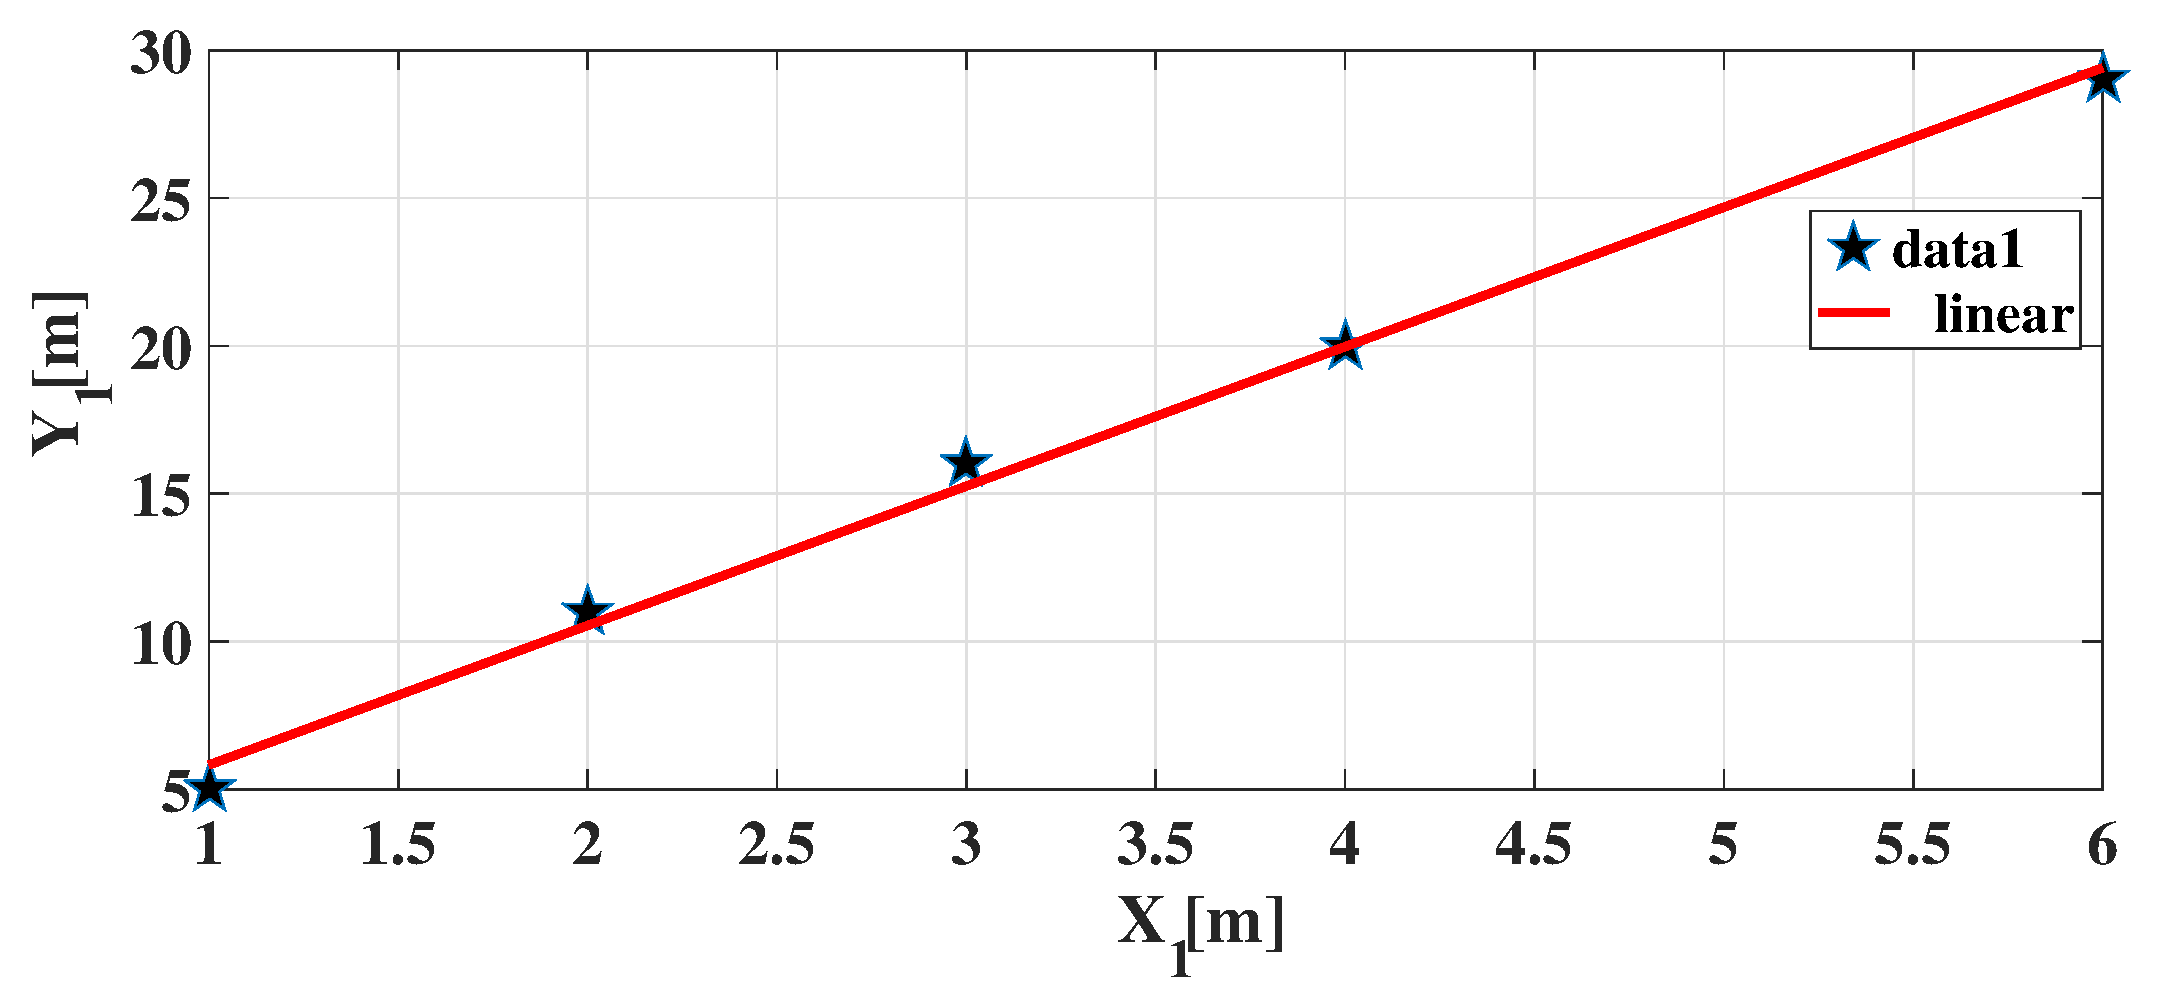
\includegraphics[scale=0.23]{fig} %[se define tamaño de la figura]{nombre del archivo con la figura}
\caption{Nombre descriptivo de la figura.} %Numera y titula la gráfica
\label{lvdt4} %Permite referenciar la grafica en el texto EJ: en la gráfica \ref{lvdt4} se observa...
\end{figure}
También puede usar rutina  generada por comandos en R en este escrito
<<>>=
x<-iris
plot(x)
@

También se pueden anexar subfiguras, modificar la posición y el tamaño. En el archivo de imagen no debe haber título. Si se desea anexar imágenes extraídas de otras fuentes (por ejemplo Internet), estas deben tener buena calidad y preferiblemente estar en formato png).

Para referenciar o nombrar una figura en el texto: En la figura \ref{lvdt4} se presenta la característica $I_1$ contra $V_1$.


%%%%%%%%%%%%%%%%%%%%%%%%%%%%%%%%%%%%%%

\section{Implementación de la solución}
En esta sección se presenta la materialización de lo que usted encontró en la investigación, se debe detallar la construcción realizada con R u otro software utilizado.

%%%%%%%%%%%%%%%%%%%%%%%%%%%%%%%%%%%%%%%%%
%%%%%%%%%%% SECCIONES FINALES %%%%%%%%%%% 
%%%%%%%%%%%%%%%%%%%%%%%%%%%%%%%%%%%%%%%%%
\section{Resultados}
En esta sección se describen  los resultados obtenidos representados mediante gráficas y tablas. Los resultados y tablas deben ser discutidos en el texto. 
%%%%%%%%%%%%%%%%%%%%%%%%%%%
%%%%%%%%% TABLAS %%%%%%%%%%
%%%%%%%%%%%%%%%%%%%%%%%%%%%
\subsection{Tablas en \LaTeX}
Para definir una tabla:

\begin{table}[H]
\centering
\caption{Nombre de la tabla}
\label{table1}
\begin{tabular}{c c c}\hline\hline
\textbf{Símbolo} & \textbf{Nombre} & \textbf{Código Latex}\\ \hline
$\alpha$ & alpha & \verb|\alpha| \\
$\mu$ & mu & \verb|\mu|\\
$\beta$ & beta & \verb|\beta|\\
$\Omega$ & Omega & \verb|\Omega| \\\hline \hline
\end{tabular}
\end{table}
Para mencionar la tabla en el documento: en la tabla \ref{table1} se muestran algunos ejemplos de código \LaTeX para obtener letras griegas\footnote{Se recomienda usar la página \url{https://www.tablesgenerator.com/}}.


%%%%%%%%%%%%%%%%%%%%%%%%%%%
%%%%%%%%%%%%%%%%%%%%%%%%%%%%%%%%%%%%%
%%%%%%%%%%%% CONCLUSIONES %%%%%%%%%%%
%%%%%%%%%%%%%%%%%%%%%%%%%%%%%%%%%%%%%
\section{Conclusiones}
En esta sección se presentan de forma clara y en tercera persona las conclusiones obtenidas respecto a la solución planteada y el desempeño del prototipo implementado.
%%%%%%%%%%%%%%%%%%%%%%%%%%%%%%%%%%%%%

\ifCLASSOPTIONcaptionsoff
  \newpage
\fi

%%%%%%%%%%%%%%%%%%%%%%%%%%
%%%%%% BIBLIOGRAFIA %%%%%%
%%%%%%%%%%%%%%%%%%%%%%%%%%
\begin{thebibliography}{1}

\bibitem{Ross}
	Ross R.. The prevention of malaria (2nd edition, with Addendum). John Murray, London. 1911.
\bibitem{Kermack}
  Kermack, W. O. and McKendrick, A. G. . A Contribution to the Mathematical Theory of Epidemics
Royal Society of London Proceedings Series A. 1927;115:700–721
\bibitem{kopka}
H.~Kopka and P.~W. Daly, \emph{A Guide to \LaTeX}, 3rd~ed.\hskip 1em plus
  0.5em minus 0.4em\relax Harlow, England: Addison-Wesley, 1999.
	
\bibitem{link}
Overleaf. \url{https://www.overleaf.com/}. Recuperado el 30 de Enero de 2017.

\bibitem{imagenes}
Youtube, canal schaparro. \url{https://youtu.be/IhvF6iY7n5k}. Recuperado el 30 de Enero de 2017.

\bibitem{dia}
Dia Diagram Editor. \url{https://sourceforge.net/projects/dia-installer/}. Recuperado el 30 de Enero de 2017.

\end{thebibliography}
%%%%%%%%%%%%%%%%%%%%%%%%%%

\end{document}
%%%%%%%%%%%%%%%%%%%%%%%%%%%%%%%%
%%%%%% FIN DEL DOCUMENTO %%%%%%%
%%%%%%%%%%%%%%%%%%%%%%%%%%%%%%%%




